\section{Descrizione del Modello}
Il modello considerato \cite{mostafizi2019agent} é un sistema multi-agente che prevede l'evacuazione da una città in caso di tsunami di auto e pedoni.
%
% TODO: riscrivere
L'evacuazione non include le conseguenze del terremoto che avviene prima dello tsunami e viene considerata iniziare alla fine di questo.

Per la distribuzione della popolazione é stato considerato uno scenario a mezzogiorno di un fine settimana di estate,
che presenta una maggiore concentrazione di residenti sulla spiaggia e nel centro della città.
%
La popolazione sulla costa e nel centro é distribuita normalmente,
mentre quella nella zona residenziale é distribuita uniformemente (Figura \ref{fig:population}).

\begin{figure}
  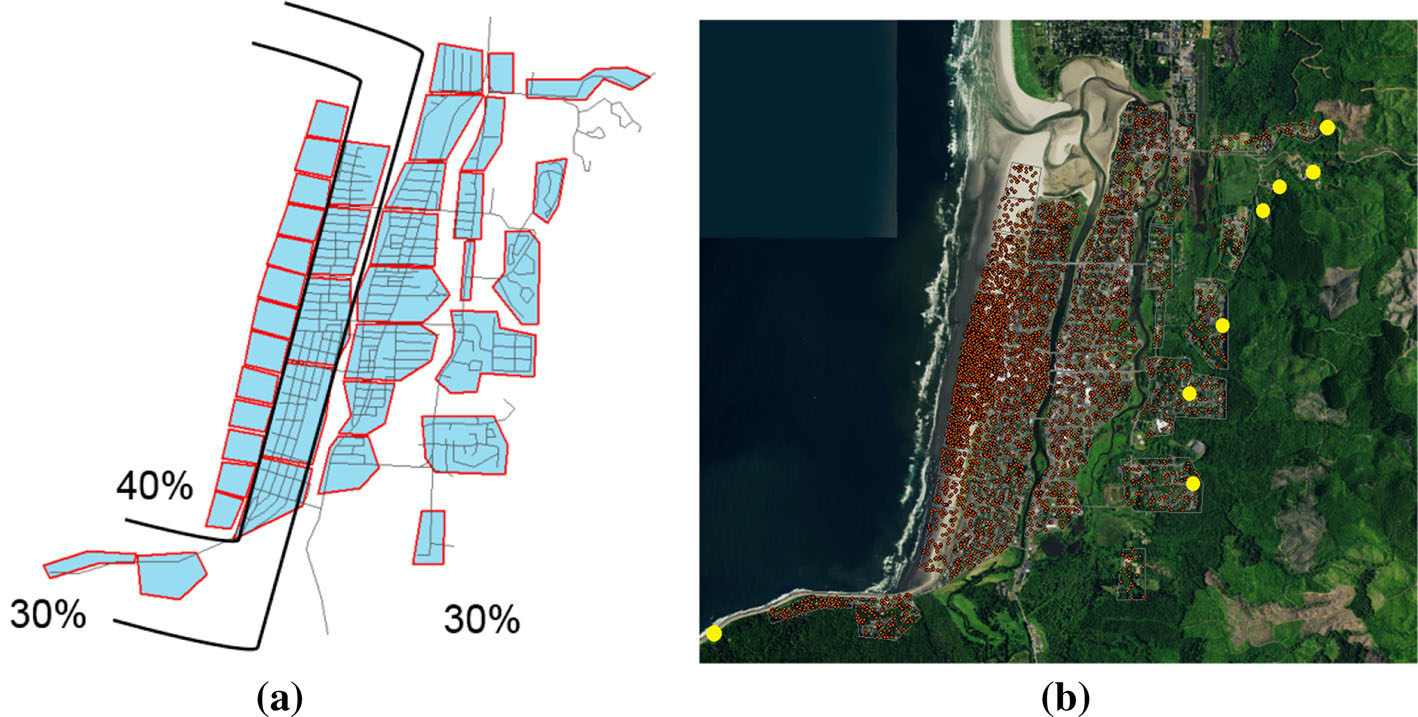
\includegraphics[width=\textwidth]{images/population}
  \caption{Distribuzione della popolazione nello scenario considerato.
    (a) Mostra le aree in cui è distribuita la popolazione, divise nelle tre macro aree: costa, centro, zona residenziale.
    (b) Immagine satellitare con la distribuzione della popolazione.}
  \label{fig:population}
\end{figure}

\subsection{Ambiente}
L'ambiente é composto dallo tsunami e da una rete stradale.

% TODO: riscrivere
Lo tsunami é rappresentato dai valori di profondità e velocità del flusso nel tempo all'interno dell'area (discretizzata in una griglia).
Un agente viene considerato vittima se l'altezza dell'onda nel punto in cui si trova é superiore o uguale a un parametro $H_c$.

La rete stradale é rappresentata da un grafo, i cui nodi corrispondono alle intersezioni e gli archi alle strade.
Tutte le strade sono considerate a senso unico, con una sola corsia e con una velocità limite di 55 km/h.
%
8 delle intersezioni sono marcate come rifugi con capacità illimitata.

% TODO: riscrivere
Gli agenti si muovono seguendo la rete stradale fino a raggiungere un rifugio.

\subsection{Agenti}
All'inizio dell'evacuazione tutti gli agenti si trovano all'esterno di edifici e auto
e autonomamente scelgono come evacuare. Le scelte sono evacuare a piedi o in auto, verticalmente o orizzontalmente.
Una volta che ogni agente decide in che modo evacuare non cambierà scelta per tutta la simulazione.

Il tempo impiegato per prepararsi all'evacuazione (milling time) é modellato tramite la distribuzione di Rayleigh.
Questo tempo comprende anche il raggiungimento del veicolo.

All'inizio della simulazione ogni agente decide come destinazione il rifugio più vicino
raggiungibile seguendo il percorso più breve (\textit{shortest path}).

Stato?
\subsubsection{Pedoni}
La velocità di camminata viene stabilita tramite una distribuzione normale
con media 1.21 m/s e deviazione standard 0.20 m/s.
La velocità di ogni pedone rimane costante durante tutta l'evacuazione.

% Non viene gestita alcuna interazione Pedone-Pedone o Pedone-Auto.

\subsubsection{Auto}
Viene considerato il caso peggiore in cui ogni auto conteniene una sola persona.

Il comportamento delle auto é modellato tramite il modello car-following, General-Motors.

\section{Estensione del Modello}
Il modello é stato esteso andando a gestire le interazioni tra gli agenti nelle intersezioni.

\subsection{Comportamento dei Pedoni}
E' stata aggiunta una variabilità nella velocità di camminata 

Marciapiedi


\subsection{Gestione degli Intersezioni}
